\section{Auswertung}
\label{sec:Auswertung}
Die in dieser Auswertung erstellten Plots werden mithilfe der \textit{Python}-Erweiterung 
\textit{matplotlib}~\cite{matplotlib} erstellt. Die Fortplanzung der Messunsicherheiten werden mithilfe von
\textit{uncertainties}~\cite{uncertainties} bestimmt und genügen der Gaußschen Fehlerfortplanzung
\begin{equation*}
    \symup{\Delta} F = \sqrt{\sum_{i}\left(\frac{\symup{d}F}{\symup{d}y_{i}}\symup{\Delta} y_{i} \right)^2}.
\end{equation*}
Die Messunsicherheiten der Zählraten $N$ sind poissonverteilt und werden daher mit $\symup{\Delta}N = \sqrt{N}$ berechnet.

\subsection{Charakteristik des GMZ}
Die Charakteristik des GMZ wird bestimmt, indem die Anzahl der pro Sekunde gemessenen Impulse in Abhängigkeit
von der anliegenden Zählrohrspannung aufgetragen wird. Hierbei lassen sich große Abweichungen einzelner Messwertgruppen
beobachten, die im Folgenden nicht weiter betrachet werden.\footnote{Dies geschieht aufgrund einer bekannten Fehlfunktion
eines Verstärkers im Versuchsaufbau. Die Auswirkungen auf den weiteren Versuch werden in Abschnitt \ref{sec:Diskussion}
ausführlich diskutiert.}

\begin{longtable}{c c c c}
    \caption{Messwerte zur Bestimmung der Charakteristik des GMZ sowie der freigesetzten Ladung. Für den Strom $I$ wird eine%
    Messunsicherheit von $\symup{\Delta} I = \qty{0.1}{\micro\ampere}$ angenommen.} \label{tab:messdaten} \\
    \hline
    {$U \mathbin{/} \unit{\volt}$} & {Zählrate} & {$N \mathbin{/} {\unit{\second}}$} & {$I \mathbin{/} \unit{\micro\ampere}$} \\
    \hline
    \endfirsthead
    \caption[]{Messwerte zur Bestimmung der Charakteristik des GMZ sowie der freigesetzten Ladung. Für den Strom $I$ wird eine%
    Messunsicherheit von $\symup{\Delta} I = \qty{0.1}{\micro\ampere}$ angenommen.(Fortsetzung)}\\
    \hline
    {$U \mathbin{/} \unit{\volt}$} & {Zählrate} & {$N \mathbin{/} {\unit{\second}}$} & {$I \mathbin{/} \unit{\micro\ampere}$} \\
    \hline
    \endhead
    \hline
    \endfoot
    330 & $\num{ 9880+- 99}$ & $\num{ 82.33+-0.83}$ & 0,1 \\
    340 & $\num{ 9994+-100}$ & $\num{ 83.28+-0.83}$ & 0,2 \\
    350 & $\num{10221+-101}$ & $\num{ 85.17+-0.84}$ & 0,2 \\
    360 & $\num{10159+-101}$ & $\num{ 84.66+-0.84}$ & 0,2 \\
    370 & $\num{10393+-102}$ & $\num{ 86.61+-0.85}$ & 0,2 \\
    380 & $\num{10326+-102}$ & $\num{ 86.05+-0.85}$ & 0,2 \\
    390 & $\num{10443+-102}$ & $\num{ 87.03+-0.85}$ & 0,2 \\
    400 & $\num{10516+-103}$ & $\num{ 87.63+-0.85}$ & 0,3 \\
    410 & $\num{10457+-102}$ & $\num{ 87.14+-0.85}$ & 0,3 \\
    420 & $\num{10719+-104}$ & $\num{ 89.33+-0.86}$ & 0,4 \\
    430 & $\num{13720+-117}$ & $\num{114.33+-0.98}$ & 0,4 \\
    440 & $\num{16377+-128}$ & $\num{136.47+-1.07}$ & 0,4 \\
    450 & $\num{16365+-128}$ & $\num{136.38+-1.07}$ & 0,4 \\
    460 & $\num{15932+-126}$ & $\num{132.77+-1.05}$ & 0,4 \\
    470 & $\num{14108+-119}$ & $\num{117.57+-0.99}$ & 0,4 \\
    480 & $\num{10787+-104}$ & $\num{ 89.89+-0.87}$ & 0,5 \\
    490 & $\num{10606+-103}$ & $\num{ 88.38+-0.86}$ & 0,5 \\
    500 & $\num{10553+-103}$ & $\num{ 87.94+-0.86}$ & 0,5 \\
    510 & $\num{10562+-103}$ & $\num{ 88.02+-0.86}$ & 0,5 \\
    520 & $\num{10617+-103}$ & $\num{ 88.47+-0.86}$ & 0,6 \\
    530 & $\num{10990+-105}$ & $\num{ 91.58+-0.87}$ & 0,6 \\
    540 & $\num{12046+-110}$ & $\num{100.38+-0.91}$ & 0,6 \\
    550 & $\num{13559+-116}$ & $\num{112.99+-0.97}$ & 0,6 \\
    560 & $\num{13181+-115}$ & $\num{109.84+-0.96}$ & 0,6 \\
    570 & $\num{10699+-103}$ & $\num{ 89.16+-0.86}$ & 0,6 \\
    580 & $\num{10575+-103}$ & $\num{ 88.12+-0.86}$ & 0,6 \\
    590 & $\num{10779+-104}$ & $\num{ 89.83+-0.87}$ & 0,6 \\
    600 & $\num{10668+-103}$ & $\num{ 88.90+-0.86}$ & 0,7 \\
    610 & $\num{10622+-103}$ & $\num{ 88.52+-0.86}$ & 0,7 \\
    620 & $\num{10611+-103}$ & $\num{ 88.42+-0.86}$ & 0,7 \\
    630 & $\num{10858+-104}$ & $\num{ 90.48+-0.87}$ & 0,7 \\
    640 & $\num{10640+-103}$ & $\num{ 88.67+-0.86}$ & 0,7 \\
    650 & $\num{10761+-104}$ & $\num{ 89.67+-0.86}$ & 0,7 \\
    660 & $\num{10878+-104}$ & $\num{ 90.65+-0.87}$ & 0,8 \\
    670 & $\num{10774+-104}$ & $\num{ 89.78+-0.86}$ & 0,8 \\
    680 & $\num{10727+-104}$ & $\num{ 89.39+-0.86}$ & 0,8 \\
    690 & $\num{11005+-105}$ & $\num{ 91.71+-0.87}$ & 0,8 \\
    700 & $\num{11160+-106}$ & $\num{ 93.00+-0.88}$ & 0,8 \\
    \bottomrule
\end{longtable}

\begin{figure}
    \centering
    \includegraphics{build/charakteristik_roh.pdf}
    \caption{Graphische Darstellung der Messwerte zur Bestimmung der Charakteristik des GMZ aus%
    \autoref{tab:messdaten}.}
    \label{fig:charakteristik_roh}
\end{figure}

In \autoref{fig:charakteristik} ist ein Bereich auszumachen, in dem die Anzahl der Impulse annähernd linear
zunimmt. Dieser Bereich wird auch Plateaubereich genannt und hat eine Länge von $L=\qty{290}{\volt}$. Mithilfe der \textit{Python}-Erweiterung \textit{scipy} \cite{scipy} wird eine lineare Ausgleichsrechnung
für die Werte in dem Plateaubereich durchführt. Für eine Ausgleichsgerade des Typs $y=mx + b$ ergeben sich die
Werte
\begin{align*}
    m &= \qty{0.0070+-0.0019}{\per\second\per\volt} & b &= \qty{85.0+-1.0}{\per\second}.
\end{align*}

\begin{figure}
    \centering
    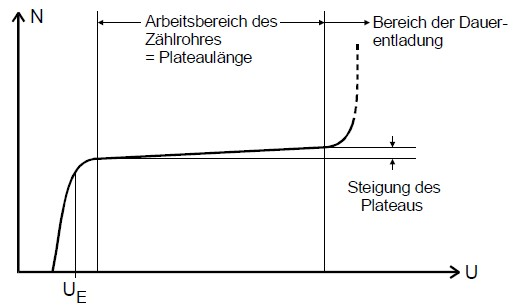
\includegraphics{build/charakteristik.pdf}
    \caption{Graphische Darstellung der Charakteristik des GMZ mit eingezeichneter Ausgleichsgerade der %
    Messwerte des Plateaus. Die in \autoref{fig:charakteristik_roh} gekennzeichneten stark abweichenden %
    Messwerte werden hierbei nicht berücksichtigt.}
    \label{fig:charakteristik}
\end{figure}





\subsection{Freigesetzte Ladung im GMZ}



\begin{figure}[H]
    \centering
    \includegraphics{build/ladung.pdf}
    \caption{Darstellung der für bestimmte Spannungen freigesetzten Ladungen im GMZ.}
    \label{fig:ladung}
\end{figure}